Benchmarking-delens fremmeste formål er at finde svar på en række spørgsmål
inden udregningen sættes igang.  Reelt har vi kun en enkelt parameter vi kan
skrue på, nemlig $m$ - antallet af dronninger vi placerer på hver board før vi
genererer et mig job til at regne videre på det board.  Hvilket forhold mellem 
\fixme{what?}
%\subsection{Takaken}
%\subsection{Java port}
%\subsection{Java port v2}
%\subsubsection{Rekursion vs. Iterativ metode}
%\subsubsection{Iterativ med checkpoints}
%\subsection{MiGrid}

\subsection{Lokale tests}

Vi starter med at teste de forskellige udgaver af koden lokalt, så vi har en
baseline at sammenligne med.

Alle lokale tests er kørt på en IBM T43, med en pentium m 1.86Ghz cpu, 

Java koden er kompilet med javac

\begin{verbatim}
alex@roadrunner:~/temp/queens/src/main/java$ javac -version
javac 1.5.0_11
\end{verbatim}

C koden er kompilet med \texttt{gcc -Os -O2 -o nq nqueens.c}

\begin{verbatim}
alex@roadrunner:~/temp/queens/src/main/java$ gcc --version
gcc (GCC) 4.1.2 (Ubuntu 4.1.2-0ubuntu4)
\end{verbatim}

De første tests er kørt på revision 77 (i forbindelse med den iterative test er
udskrivning af debug info til skærmen dog blevet kommenteret ud)

\begin{figure}[h]
\begin{center}
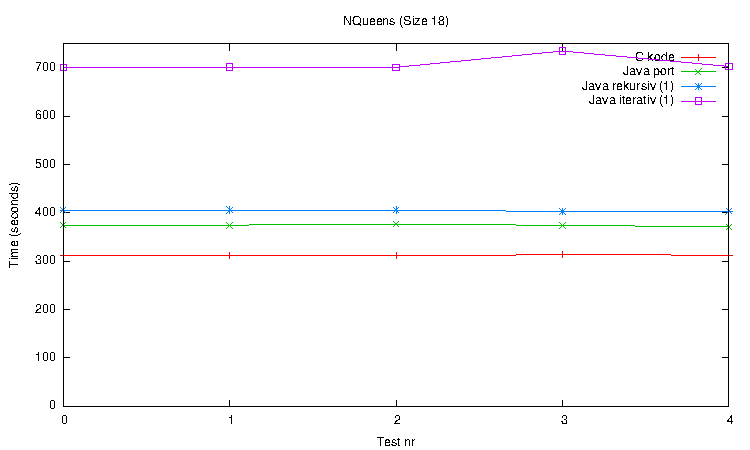
\includegraphics{../benchmarks/b1.pdf}
\caption{insert proper caption here } 
\label{plot:b1}
\end{center}
\end{figure}

Som det ses er C udgaven en smule hurtigere end den direkte java port, der igen
er lidt hurtigere end den paralleliserede udgave af koden, når den kører
rekursivt. Den iterative udgave er væsentlig langsommere..

Den parallelle udgave af koden er i dette tilfælde her kørt med
\texttt{maxSteps} på 1. 

Den næste graf er den rekursive udgave af den parallele kode kørt med forskellig
\texttt{maxSteps}. 

\begin{figure}[h]
\begin{center}
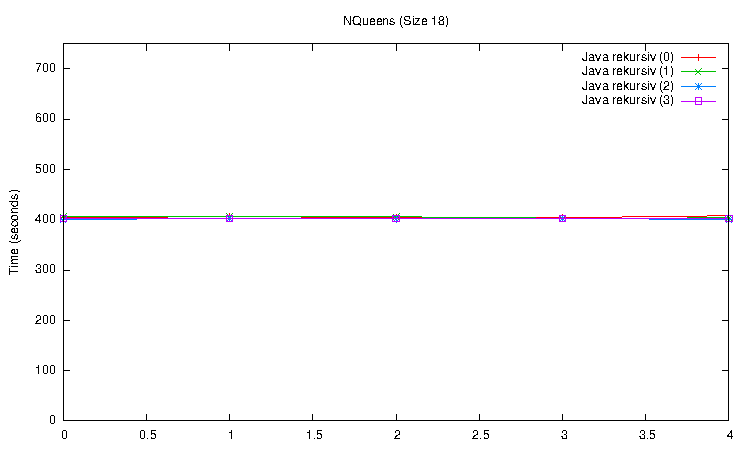
\includegraphics{../benchmarks/b2.pdf}
\caption{insert proper caption here } 
\label{plot:b2}
\end{center}
\end{figure}

Som det ses, har det ikke den store indflydelse på performance, når det kører
lokalt, der er altså ikke det store overhead ved at generere en masse opgaver og
løse dem bagefter, når det kører lokalt. 

Det skal også nævnes at for $maxSteps>n/2$ vil vores program regne forkert.
Dette skyldes \fixme{ja.. hvad skyldes det.. }

\fixme{hvor mange jobs bliver der lavet for de forskellige maxsteps, indsæt
tabel?}

Alle tests er i første omgang kørt 5 gange, dette blev gjort for at se om
køretiden svingede meget, da dette ikke lader til at være tilfældet vil resten
af testene kun blive kørt 1 gang.. 

Nu skal vi så se på hvor hurtigt det kører når vi smider det efter MiGrid. 
Disse tests er kørt med \texttt{maxSteps} 0 og 1.

\fixme{indsaet en graf, eller bare resultaterne og henvis til b3?}
De foregående tests er kørt med kode der bruger \texttt{int} til at gemme resultaterne,
i de næste tests er \texttt{int} skiftet ud med \texttt{BigInteger} (revision
83
\clearpage
Sammenligning af alle benchmarks

\begin{figure}[h]
\begin{center}
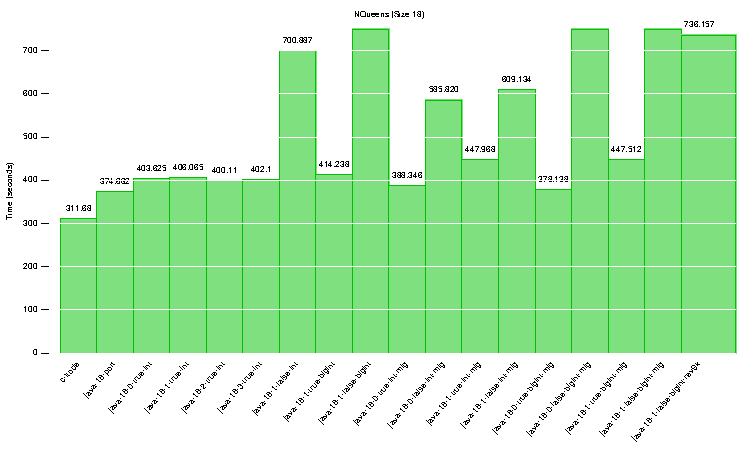
\includegraphics{../benchmarks/b3.pdf}
\caption{insert proper caption here } 
\label{plot:b3}
\end{center}
\end{figure}

Som det ses på figur \ref{plot:b3} kører den iterative udgave af koden fra
rev. 83 utroligt langsomt i forhold til foregående udgaver. 
Dette skyldes en en linje kode, der ikke var blevet kommenteret ud. Denne linje
konkatenerede to strenge. Uden denne linje kører koden væsentlig hurtigere, som
det ses af søjle 18. Den rekursive kode kører en smule langsommere med
\texttt{BigInteger} (søjle 4 mod søjle 8)

\begin{itemize}
\item[1] Takakens C-kode
\item[2] Direkte java port
\item[3] Parallel java port, \texttt{maxSteps}=0, rekursiv, int, lokal
\item[4] Parallel java port, \texttt{maxSteps}=1, rekursiv, int, lokal
\item[5] Parallel java port, \texttt{maxSteps}=2, rekursiv, int, lokal
\item[6] Parallel java port, \texttt{maxSteps}=3, rekursiv, int, lokal
\item[7] Parallel java port, \texttt{maxSteps}=1, iterativ, int, lokal
\item[8] Parallel java port, \texttt{maxSteps}=1, rekursiv, bigint, lokal
\item[9] Parallel java port, \texttt{maxSteps}=1, iterativ, bigint, lokal
\item[10] Parallel java port, \texttt{maxSteps}=0, rekursiv, int, MiG
\item[11], Parallel java port, \texttt{maxSteps}=0, iterativ, int MiG
\item[12], Parallel java port, \texttt{maxSteps}=1, rekursiv, int, MiG
\item[13], Parallel java port, \texttt{maxSteps}=1, iterativ, int, MiG
\item[14], Parallel java port, \texttt{maxSteps}=0, rekursiv, bigint, MiG
\item[15], Parallel java port, \texttt{maxSteps}=0, iterativ, bigint, MiG
\item[16], Parallel java port, \texttt{maxSteps}=1, rekursiv, bigint, MiG
\item[17], Parallel java port, \texttt{maxSteps}=1, iterativ, bigint, MiG
\item[17], Parallel java port, \texttt{maxSteps}=1, iterativ, bigint, rev9x 
\fixme{indsaet sidste tests her og opdatere graph}
\end{itemize}

\subsection{overhead ved jobskifte}

I MiG\_main() metoden i NQueenJob laver vi et timestamp i starten og slutningen af metoden. 
og kan så tage start tiden for et job og trække sluttiden for det foregående job
fra, og man har så et estimat for hvor lang tid et jobskifte tager, vi har gjort
dette for 8 jobs, og får så 7 estimater, gennemsnittet af dem bliver 18.455 sek. 
Op til 15 af disse 18 sekunder, skyldes at oneclick applet'en sover i 15 sekunder. 
Ved en kørsel med $n=18$ og $maxSteps=1$, hvor vi så får 289 jobs, giver det
knap 89 minutter. 

\subsection{kald til backtrack}
Hvis man ser på antallet af kald til backtrack de forskellige versioner laver, er de
ens for c koden og den direkte java port, og hvis man kører med $maxSteps=0$ er
antallet af kald for den parallele og iterative kode også det samme som
for c koden. Med $maxSteps>0$ får vi færre kald til backtrack, hvilket skyldes
at en del af disse kald bliver lavet i forbindelse med oprettelsen af de ekstra
boards. 
